\section{Stati monofase: equazioni di stato e trasformazioni}
Le sostanze nello stato monofase possono schematicamente essere suddivise in sostanze nello
stato aeriforme, liquido o solido. I modelli di equazioni di stato sono, in prima
approssimazione, ricondotti a modelli ideali o modelli reali.
\subsection{Gas ideali}
Le equazioni di stato dei \textbf{gas ideali} sono:
\[
    PV=MR^*T
\]
\[
    U=U(T) \;\;\;\;\;\;\;\;\;\;\;\;\Delta U = M c_V \Delta T \rightarrow \Delta u = c_V \Delta T
\]
La costante $R^*$ rappresenta la costante del gas ed è determinabile con la relazione:
\[
    R^* = \frac{R}{M_m}
\]
\[
    R=8314 [J/kmole K] =\text{costatne universale dei gas}\; \;\;\;\;\;\;\;\;\;\;M_m = \text{massa molare}\;
\]
\begin{center}
    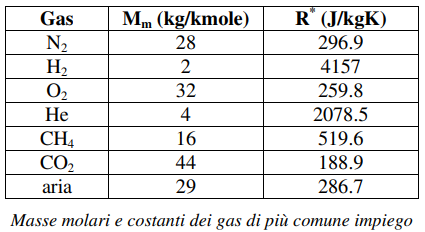
\includegraphics[height=3cm]{../NOTE SUGLI ESERCIZI/img1.PNG}
\end{center}
La grandezza $c_V$ rappresenta il calore specifico a volume costante funzione del gas e della sua
struttura molecolare. Qualora il calore specifico a volume costante possa assumersi indipendente dalla temperatura (e quindi costante) si parla di gas perfetto.
\subsection{Liquidi e solidi incomprimibili ideali}
Le equazioni di stato dei fluidi incomprimibili ideali (liquidi e solidi) sono:
\[
    v = costante
\]
\[
    U=U(T)  \;\;\;\;\;\;\;\;\;\;\;\;\Delta U = M c \Delta T \rightarrow \Delta u = c \Delta T
\]
dove $c$ è il calore specifico della sostanza.
\subsection{Gas reali}
Una possibile equazione di stato dei gas reali è:
\[
    Pv = ZRT
\]
dove $Z$ è il fattore di compressibilità. Tale coefficiente è determinabile attraverso il diagramma generalizzato che riposta il fattore di compressibilità in funzione della pressione e della temperatura ridotta. La pressione e la temperatura ridotte sono valori adimensionali ottenuti dalle relazioni:
\[
    P_R = \frac{P}{P_{cr}} \;\;\;\;\;\;\;\;\;\;\;\;\;\;\;T_R = \frac{T}{T_{cr}}
\]
in cui $P_{cr}$ e $T_{cr}$ rappresentano i valori di pressione e temperatura nello stato critico.
\begin{center}
    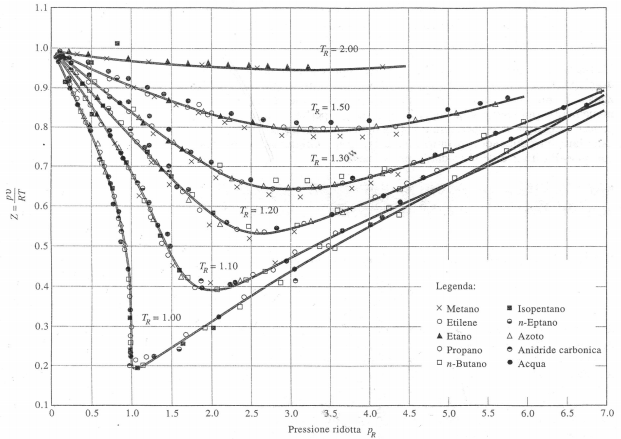
\includegraphics[height=5cm]{../NOTE SUGLI ESERCIZI/img2.PNG}
\end{center}
\subsection{Liquidi e solidi reali}
Le equazioni di stato dei liquidi e solidi reali sono formulate in forma differenziale:
\[
    dv = \beta v \cdot dT - K_Tv \cdot  dP
\]
\[
    \text{Coefficiente di dilatazione termica isobaro}\;\;\;\beta = \frac{1}{v} \left(\frac{\delta v}{\delta T}\right)_P
\]
\[
    \text{Coefficiente di comprimibilità isotermo}\;\;\;K_T = - \frac{1}{v} \left(\frac{\delta v}{\delta P}\right)_T
\]
Siccome $\beta$ e $K_T$ possono essere considerati costanti per ampi intervalli di temperatura e di pressione, la precedente relazione differenziale è integrabile e lo stato calcolabile.
\begin{center}
    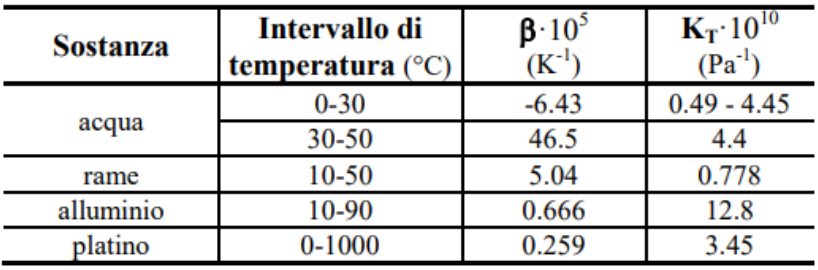
\includegraphics[height=3cm]{../NOTE SUGLI ESERCIZI/img3.PNG}
\end{center}
\subsection{Trasformazioni politropiche}
Le \textbf{trasformazioni politropiche} sono trasformazioni termodinamiche \textbf{internamente reversibili}
proprie dei \textbf{gas perfetti} e caratterizzate dall’avere un calore specifico $c_x$ \textbf{costante}.\newline
\newline
L’equazione della politropica in coordinate P,v risulta
\[
    Pv^n = costante \;\;\;\;\;\;\;\;\;\;\text{dove \textbf{l'indice della politropica} è}\;\;\;n = \frac{c_x - c_P}{c_x - c_V}
\]
Con l’ausilio dell’equazione di stato dei gas ideali è possibile ottenere espressioni
dell’equazione della politropica in coordinate T,P e T,v: 
\[
    P^{1-n}T^n = costante
\]
\[
    Tv^{n-1} = costante
\]
Si distinguono alcune trasformazioni elementari particolarmente utili tra le politropiche: 
\begin{center}
    \begin{tabular}{ |c|c|c|c| } 
        \hline
        Trasformazione & $c_x$ & $n = \frac{c_x - x_P}{c_x - c_V}$ \\
        \hline
        Isoterma ($T = costante$) & $\pm \infty$ & $1$ \\ 
        Isocora ($v = costante$) & $c_V$ & $\pm \infty$\\ 
        Isobara ($P = costante$) & $c_P$ & $0$\\ 
        Adiabatica ($q = costante$) & $0$ & $k= \frac{c_P}{c_V}$\\ 
        \hline
    \end{tabular}
\end{center}
\ \newline
Si ricorda che il \textbf{primo principio} è \textbf{sempre applicabile} ed essendo la trasformazione \textbf{quasi statica} vale inoltre sempre:
\[
    Q = \int_{1}^{2}TdS \;\;\;\;\;\;\;\;\;\;\;\;\;\;\;L=\int_{1}^{2}PdV
\]
Per la trasformazione \textbf{isoterma} (cioè con $n = 1$) il calore e il lavoro diventano:
\[
    Q = MT(s_2-s_2) \;\;\;\;\;\;\;\;\;\;\;\;\;\;\; L = P_1V_1 ln \left(\frac{V_1}{V_2}\right)
\]
Per le trasformazioni \textbf{isocore, isobare e adiabateche} (cioè con $n \neq 1$), invece, il calore e il lavoro diventano:
\[
    Q= Mc_x (T_2-T_1) \;\;\;\;\;\;\;\;\;\;\;\;\;\;\; L = \frac{P_1V_1}{n-1}\left[ 1 - \left(\frac{V_1}{V_2}\right)^{n-1}\right]
\]
Si suggerisce di ricorrere al calcolo degli integrali per determinare il lavoro e il calore
scambiato soltanto quando strettamente necessario. Essendo questi due termini comunque
legati tra loro dalla equazione di bilancio energetico. 
